\section{Experimental Evaluation}
\label{sec:simulation}

To demonstrate the feasibility of SemiAIM as well as evaluate the
hypothesis that SemiAIM can offer substantial improvements over
traffic signals and FCFS-Signal, we conducted a series of experiments
with the modified AIM4 simulator that simulates the behavior of
vehicles using the constraint-based reservation system.  The
implementations of fully autonomous vehicles (Type A) and human-driven
vehicles (Type H) are as provided with the simulator and described
in~\cite{bib:Dresner08Multiagent}.  The concrete implementations of
the semi-autonomous vehicles, as described in
Section~\ref{sec:vehicles}, are as follows.

\begin{small_ind_s_itemize}

\item \textbf{Type SA-ACC Vehicles}: If there exists a vehicle ahead
which is either autonomous or semi-autonomous and is going in the same
direction, it sends an anchor request to the IM.  If the request is
confirmed, the vehicle follows the vehicle ahead and enters the
intersection.  If the request is denied or there is no such vehicle
ahead, the vehicle follows rules for Type SA-CC Vehicles, shown below.

\item \textbf{Type SA-CC Vehicles}:
Sends a constant-velocity request to the IM when it is close
enough to the intersection. If it can enter the intersections by
keeping the current velocity, the request is confirmed; otherwise, the
vehicle follows rules for Type SA-C-om Vehicles, shown below.

\item \textbf{Type SA-Com Vehicles}:
Sends a whole-row request to the IM.  If the entire lane is
available, the request is confirmed; otherwise, the vehicle resends the
request after a few seconds, and at the same time decelerates enough to
be able to stop before the intersection. 
If it keeps failing to obtain a reservation it stops at
the intersection and returns control to the human driver, who must
then obey the traffic signal.
\end{small_ind_s_itemize}

Our experiments were conducted in a 3x3 intersection (3 lanes
in each direction) as shown in Figure~\ref{fig:simulator}.  Unless otherwise specified, the simulator spawns vehicles in each lane according
to a Poisson distribution with an expectation of 360 vehicles per
hour.  We denote this setting as traffic level = 360
vehicles/hour/lane.  We chose this traffic level as being heavy enough
to cause significant delays at signals, but light enough to allow for
benefits even if cars are not precisely
controlled. 

% We assume the intersection is fully observable to the
% intersection manager.

The performance of an intersection is measured by the \emph{average
delay}, where delay is computed as the increase in travel time
compared to traversing the intersection without slowing down at all,
as if no other vehicles were on the road. Thus, lower delays
correspond to better performance.  This measure is the same one used
in \cite{bib:Dresner08Multiagent}. For all the vehicles, both the
static buffer and the edge time buffer are 0.25 meters (see
\cite{bib:Dresner08Multiagent} for details), when auto-controlled.

Traffic signals are used as a fallback strategy when vehicles cannot
get a reservation.  We used an \emph{optimized} 6-phase signal
schedule that includes relatively long green times (roughly 35
seconds) for East-West and North-South phases, and shorter phases for
each of the four single direction phases (roughly 9 seconds). It was
optimized using SYNCHRO, a commercial traffic optimization package.

% According to this plan, there is a 30
% second green phase for traffic coming from East and West, followed by
% a 3 second yellow phase and a 5 second red phase.  Then, there is a 8
% second green phase for traffic from South direction only, followed by
% a 3 second yellow phase and a 5 second red phase, etc.  The timing of
% all phases is shown in Table~\ref{table:phase}.

% Traffic signals are used as a fallback strategy when
% (semi-)autonomous vehicles cannot get a reservation.  We used an
% \emph{optimized} phase plan for traffic signals in
% Table~\ref{table:phase}, which is generated by SYNCHRO, a commercial 
% traffic optimization package.  According to this plan, there is a 30
% second green phase for traffic coming from East and West, followed by
% a 3 second yellow phase and a 5 second red phase.  Then, there is a 8
% second green phase for traffic from South direction only, followed by
% a 3 second yellow phase and a 5 second red phase, etc.  The timing of
% all phases is shown in Table~\ref{table:phase}.

% \commentp{I still don't understand why the optimized phase plan is assymetric.  If there is the same traffic level in all directions, then why would a phase be longer in some directions than others???}

% \begin{table}
% \caption{The optimized phase plan for traffic signals.}
% \label{table:phase}
% \centering
% \small
% \begin{tabular}{|l|c|c|c|}
% \hline
% Direction & Green Phase & Yellow Phase & Red Phase \\
% \hline
%   East-West & 30s & 3s & 5s \\
%   South & \ 8s & 3s & 5s \\
%   East & 10s & 1s & 5s \\
%   North-South & 40s & 3s & 5s \\
%   West & 10s & 1s & 5s \\
%   North & \ 8s & 3s & 5s \\
% \hline
% \end{tabular}
% \end{table}

\subsection{Experiment 1: Technology Penetration}

Our first experiment studies the effect of an increasing penetration rate
of vehicular automation technology.  Suppose human-driven vehicles are
gradually replaced by a particular type of semi-autonomous vehicle or
fully autonomous vehicle until all vehicles become that type.  We examine how
much benefit SemiAIM provides during the transition period.

In this experiment, the traffic consisted of one of the three types of
vehicles we defined in Section~\ref{sec:vehicles} as well as Type A
and Type H vehicles.  We measured the traffic delay as we gradually
increased the ratio of (semi-)autonomous vehicles to human-driven
vehicles (Type H) while keeping the traffic level at 360
vehicles/hour/lane.  As an example, consider the ratio of Type SA-ACC
vehicles.  At the beginning, there are 0\% Type SA-ACC vehicles and
100\% human-driven vehicles, and the ratio is 0.  As the number of
Type SA-ACC vehicles increases, the ratio increases and eventually
becomes 1, which means there are 100\% Type SA-ACC vehicles and 0\%
human-driven vehicles.  We repeated the simulation 30 times for 1800s
during each time.  For each run, we measured the average delay of all
vehicles.  The average delays are shown in Figure~\ref{fig:two360}.
Each data point in the figure is an average of 30 values, and the
error bar is the 95\% confident interval of the average delay.
 
% , and the average delay is the same as Type
% H's.  When the ratio is 1, the traffic has 100\% SA-ACC vehicles and
% 0\% human-driven vehicles, and the average delay is 22.4s.

% When the
% ratio is 0.6, the traffic has 60\% SA-ACC vehicles and 40\%
% human-driven vehicles, and the average delay is 32.9s.  


\begin{figure}
\centering
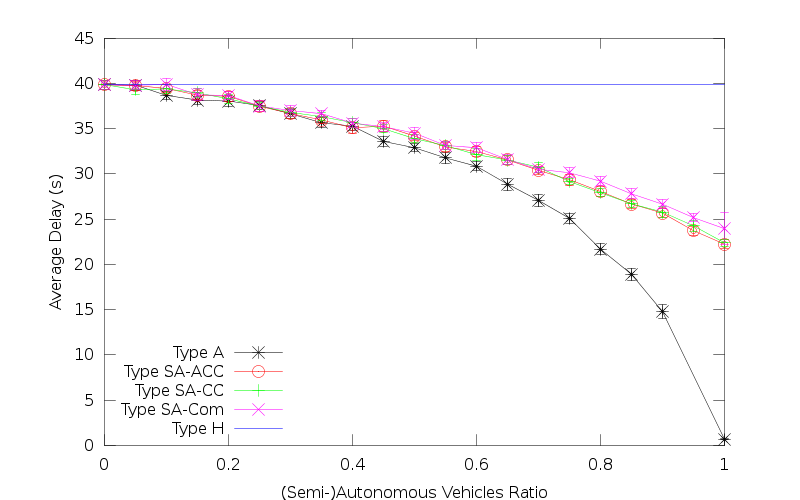
\includegraphics[width=0.9\columnwidth]{figures/figure_1.png}
\caption{(Semi-)Autonomous vehicles vs. Human-Driven vehicles. Traffic
level = 360 vehicles/lane/hour.}
\label{fig:two360}
\vspace{-.2in}
\end{figure}

According to Figure~\ref{fig:two360}, the performance of
semi-autonomous vehicles is very similar to fully autonomous vehicles
when the ratio to human-driven vehicles is below 40\%.  However, when
the ratio increases beyond 40\%, fully autonomous vehicles
increasingly outperform semi-autonomous vehicles.
% Previous studies
% showed that FCFS-Signal needs at least 90\% of fully autonomous
% vehicles in the traffic in order to be fully
% effective~\cite{bib:Dresner07Sharing}.  We successfully replicate the
% result, observing that the average delay drops rapidly when the
% traffic has more than 90\% fully autonomous vehicles, and approaches
% zero when all vehicles are fully autonomous.  Semi-autonomous vehicles
%cannot achieve the same dramatic decrease in traffic delay
We can also observe that 
with the help of SemiAIM, manage to reduce the delay by 46\% (from
39.9s to 22.4s) compared to human-driven vehicles.  As expected, in
the presence of semi-autonomous vehicles, SemiAIM provides significant
advantages even when there are no fully autonomous vehicles on the
road.

%Semi-autonomous traffic cannot perform as well as fully autonomous
%traffic under SemiAIM, but it is reasonable because the goal of
%SemiAIM is not to replace AIM, but rather to provide many of its
%benefits prior in the time period between today, when most cars are
%driven fully manually, and the time when all cars are fully
%autonomous.  To do so, it leverages features of semi-autonomy, that we
%expect will be widespread much sooner than full autonomy.

Another observation is that both Type SA-ACC and Type SA-CC vehicles
have a significantly lower average delay than Type SA-Com vehicles.
The difference is consistent with our hypothesis that the use of more
constrained requests can increase the performance of intersections
since the footprints of the vehicles are smaller and more vehicles can
enter the intersection at the same time.  Nonetheless, the difference
is small because the simulated human drivers in the simulator can
control their vehicles quite well.

% In reality the difference actually depends on some human drivers needs
% to reserve a large number of tiles, causing a decrease of the traffic
% delay when all vehicles are human-driven.  assumption we made on how
% well human drivers perform. In our simulations,

% This result confirms our hypothesis that while semi-autonomous
% vehicles can significantly bridge the gap between the time when all
% vehicles are human-driven to that when most are autonomous, there will
% likely always remain strong benefits of full autonomy, especially at
% high traffic levels.  



% It is true that semi-autonomy would not ``harm'' normal traffic which
% follows traffic signals, but they have almost no chance to enter the
% intersection in phases other than when the signal is green. This
% condition leads to little or no improvement over traditional traffic
% light policy.



% However, the average delay of
% semi-autonomous vehicles cannot be reduced to nearly zero.  When all
% vehicles are semi-autonomous, the average delay (22.4s) is roughly
% half of the average delay for human-driven vehicles only (39.9s).  

% The last observation is that 
% if there are less than 80\% of vehicles
% that are fully autonomous and more than 20\% of vehicles that are
% human-driven, it is still possible to form a team of semi-autonomous
% vehicles that performs better. Thus, we need at 80\% of fully
% autonomous vehicles in order to guarantee the benefit.

% We expect that
% in the presence of semi-autonomous vehicles, SemiAIM
% will provide significant advantages over FCFS-Signal if we assume that
% semi-autonomous vehicles have to act as fully human-driven vehicles in
% FCFS-Signal.  

% The experiments only compare two types of vehicles at the same
% time---human-driven vehicles (Type H) and the type of vehicles
% specified in the legends.

% As described in the
% legend, the traffic level is 360 vehicles/hour/lane, so it can be
% easily calculated how many vehicles of a certain type are spawned in
% each lane.

% Another observation is that the average delay when all vehicles are
% semi-autonomous (i.e., the ratio is 1) is approximately equal to the
% average delay of fully autonomous vehicles when the ratio is 0.8
% (i.e., 80\% of vehicles are fully autonomous and the remaining 20\%
% are human-driven). Thus 

% Another observation is that if there are less than 80\% of vehicles
% that are fully autonomous and more than 20\% of vehicles that are
% human-driven, it is still possible to form a team of semi-autonomous
% vehicles that performs better. Thus, we need at 80\% of fully
% autonomous vehicles in order to guarantee the benefit.

% To demonstrate the feasibility of SemiAIM as well as evaluate the
% hypothesis that SemiAIM can offer substantial improvements over
% traffic signals and FCFS-Signal,


\subsection{Experiment 2: Incremental Deployment}

Our second experiment considers realistic scenario of
\emph{incremental deployment} of autonomous vehicle technology.  We
believe that the adoption of semi-autonomous vehicles will be much
faster than fully autonomous vehicles since the cost of ownership of
semi-autonomous vehicles are lower.  Thus we anticipate there will be
a period of time during which semi-autonomous vehicles dominate the roads.
However, this domination will be short-lived---eventually fully autonomous
vehicles will displace semi-autonomous vehicles due to their greater
 convenience.  This section studies the
effects of different levels of incremental deployment of
(semi-)autonomous vehicles over time.

We consider two plausible deployment schedules, one for the period of
time before the domination of semi-autonomous vehicles, and the other
for the subsequent period.  In the first deployment schedule
(Table~\ref{table:3}), Type H vehicles on the road are gradually
displaced by (semi-)autonomous vehicles.  Assume two out of three car
buyers who abandoned their vehicles for newer technology will buy a
semi-autonomous vehicles rather than a fully autonomous vehicle.  Then
eventually about two thirds of vehicles on the road will be
semi-autonomous, and one third will be fully autonomous.
Table~\ref{table:4} shows the second deployment schedule under which
semi-autonomous vehicles are gradually replaced by fully autonomous
vehicles. We assume that even when most vehicles are fully autonomous,
a small number of drivers still prefer driving themselves.

\begin{table}[t]

\caption{The deployment schedule in Figure~\ref{fig:figure3}.}
\label{table:3}
\centering
\small
\begin{tabular}{|c|c|c|}
    \hline
    Type H&  Type SA-ACC / SA-CC / SA-Com &    Type A\\
    \hline
    90\% &      \ 9\% &   \ 1\% \\
    \hline
    87\% &     11\% &    \ 2\% \\
    \hline
    84\% &     13\% &    \ 3\% \\
    \hline
     ...&   ...&   ...\\
    \hline
    \ 0\%&     69\% &  31\% \\
    \hline
\end{tabular}

\mbox{}

\caption{The deployment schedule in Figure~\ref{fig:figure4}.}
\label{table:4}
\centering
\small
\begin{tabular}{|c|c|c|}
    \hline
     Type H&  Type SA-ACC / SA-CC / SA-Com &    Type A\\
    \hline
     10\%&     85\%&   \ 5\% \\
    \hline
     10\%&     80\%&  10\% \\
    \hline
     10\%&     75\%&  15\% \\
    \hline
      ...&  ... &  ...\\
    \hline
     10\%&       5\%&  85\% \\
    \hline
\end{tabular}
\vspace{-.3in}
\end{table}

Figures~\ref{fig:figure3} and \ref{fig:figure4} show the results of
the simulations according to these deployment schedules.  The
simulation setup is exactly the same as in Experiment 1.
For each vehicle distribution, we ran the simulation 30 times for 1800s each run.  Thus, each data point in the figures is
an average of 30 delay times.  The 95\% CIs of the average are shown
as the error bars in the figures.  According to these figures, the
average delay of the vehicles keeps decreasing as
(semi-)autonomous vehicles are deployed, and the choice of the
semi-autonomous vehicle technology does not matter much.  Ultimately, the
average delay depends on the number of drivers who insist on driving
themselves.

\begin{figure}[t]

\centering
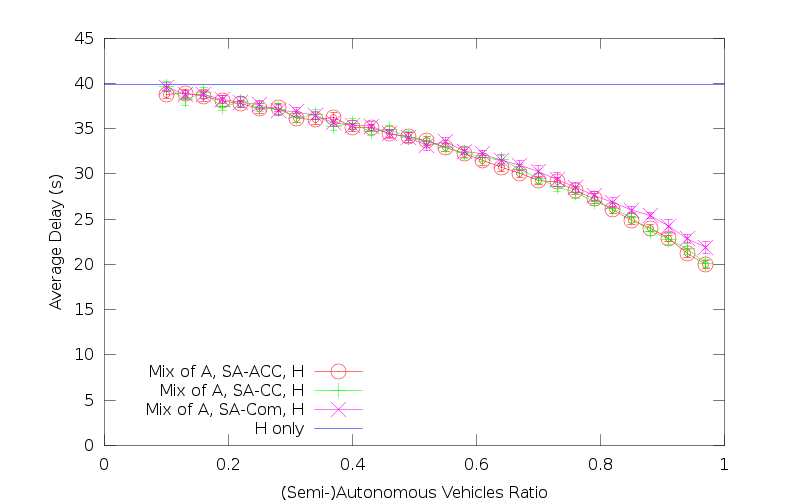
\includegraphics[width=0.9\columnwidth]{figures/figure_3.png}
\caption{The average delay according to the 
deployment schedule in Table~\ref{table:3}.
Traffic level = 360 vehicles/lane/hour.}
\label{fig:figure3}

\mbox{}

\centering
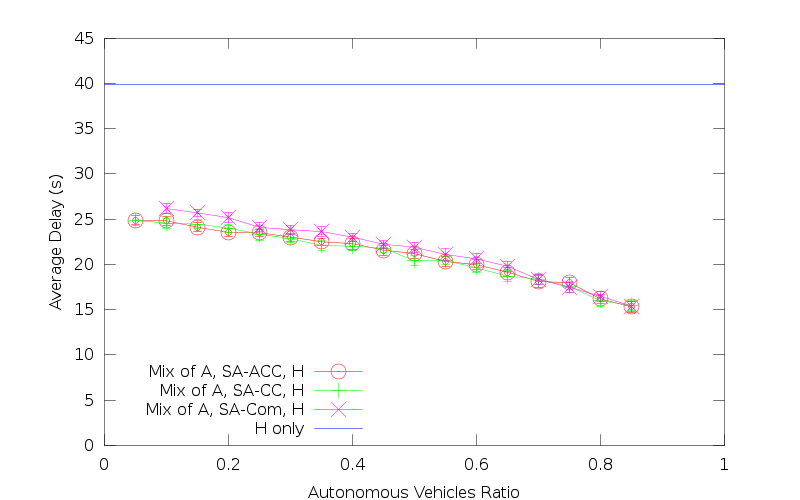
\includegraphics[width=0.9\columnwidth]{figures/figure_4.png}
\caption{The average delay according to the 
deployment schedule in Table~\ref{table:4}.
Traffic level = 360 vehicles/lane/hour.}
\label{fig:figure4}
\end{figure}


% Our second experiment evaluates the performance of SemiAIM in a
% traffic with a mixture of all three types of vehicles: Type A, Type H,
% and one of Types SA-ACC, SA-ACC, and SA-Com.  We conducted two
% experiments: 1) gradually shifting from human-driven vehicles to
% autonomous and semi-autonomous vehicles, and 2) shifting from
% semi-autonomous vehicles to fully autonomous vehicles.  The schedule
% for shifting is indicated in Tables~\ref{table:3} and~\ref{table:4},
% which can be used to interpret the mix of vehicles along the x-axes of
% Figures~\ref{fig:figure3} and~\ref{fig:figure4} respectively.


% \begin{enumerate}

% \item Gradually replace human-driven vehicles with semi-autonomous
%   vehicles. The result shows that with the appearance of more autonomous
%   and semi-autonomous vehicles (i.e.\ fewer human-driven vehicles), the
%   delay time decreases. The result is shown in
%   Figure~\ref{fig:figure3}.

% \item Gradually replace semi-autonomous vehicles with fully autonomous
%   vehicles. The result shows that when the percentage of human
%   vehicles is fixed, the delay time decreases with appearance
%   of more autonomous vehicles (i.e.\ fewer semi-autonomous vehicles).
%   The result is shown in Figure~\ref{fig:figure4}.

% \end{enumerate}


% since
% if a vehicle keep failing to obtain a reservation,
% it will try to send a whole-row request.

% For example, unlike SA-CC, the vehicles that make constant-velocity
% requests will not issue another constant-velocity requests after it
% fails to obtain a reservation; instead, it will send a whole-row
% request.


% We think it has a lot to do
% with whether vehicles can actually get a reservation.  Vehicles using
% anchor requests may not find another vehicles to follow, and vehicles
% using constant-velocity requests may not find a trajectory that can
% pass the intersections at constant velocity without hitting other
% vehicles. 

% The performance of semi-autonomous vehicles can be significantly
% better than human-driven vehicles in low traffic levels. However, the
% benefits decrease at higher traffic levels.  In
% Figure~\ref{fig:request540}, we increase the traffic level to 540
% vehicles/hour/lane.  At this traffic level, congestion appears more
% often, causing a large increase of traffic delay in all cases except
% one: \emph{all} vehicles are fully autonomous.  While the average
% delay for Type SA-ACC and Type SA-CC vehicles are significantly lower
% than human-driven vehicles when the ratio is close to 1, they yields
% less than 15\% decrease in traffic delay, which is much smaller than
% the 46\% decrease of traffic delay at the traffic level of 360
% vehicles/lane/hour.  Even worse, the average delay of Type SA-Com
% vehicles is higher then Type H Vehicles, meaning that drivers of
% SA-Com vehicles are better not to use the reservation system but
% follow the traffic signals at the intersection.  These results
% highlighted the fact that SemiAIM may not work well at medium or high
% traffic level. But the result could be better if we can devise
% semi-autonomous vehicles with more powerful autonomy features than
% simple and adaptive cruise control.  Nevertheless, for lower levels of
% traffic, the benefits of semi-autonomy can be large.

%%%%%%%%%%%%%%%%%%%%%%%%%%%%%%%%%%%%%%


% \commentp{If we end up with more space to use, it would be good to do
% one or two experiments along the lines of the future work mentioned in
% the last paragraph of the paper. - what happens if there are different
% amounts of traffic in different directions?}
% \commentn{This is mentioned in the future work.}


% To demonstrate the feasibility of SemiAIM as well as evaluate the
% hypothesis that SemiAIM can offer substantial improvements over
% traffic signals and FCFS-Signal, we modified the AIM4 simulator at
% \url{http://www.cs.utexas.edu/~aim} to simulate the behavior of
% vehicles in the constraint-based reservation system and measured the
% average delays of vehicles under (1) AIM, (2) SemiAIM, and (3) traffic
% signals with optimized signal timing.

% \begin{figure}[t]
%   \centering
%   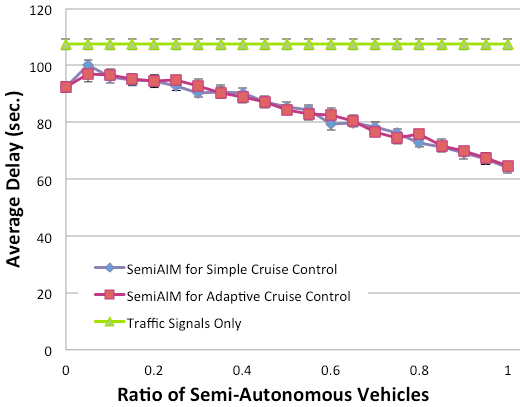
\includegraphics[width=2.4in]{figures/figure2}
%   \caption{Average delay vs. the ratio of semi-autonomous vehicles
% to human-controlled vehicles. T.
%     L. = 720 veh./hour/lane.}
%   \label{fig:two360}
%   \vspace{-.1in}
% \end{figure}

% The experiments were conducted in a $3 \times 3$ intersection.  In the first
% experiment, the traffic consisted of human-controlled vehicles and
% fully autonomous vehicles only. We gradually increased the percentage
% of autonomous vehicles while keeping the traffic level at 720
% vehicles/hour/lane. We compared two variants of SemiAIM with optimized
% traffic signals in which all vehicles must follow the traffic signals.
% Figure~\ref{fig:figure1} shows that as the number of autonomous
% vehicles increases, the average delay decreases. In particular, when
% most vehicles are autonomous, the average delay is close to zero.  In
% the second experiment, we created a traffic consisting of
% human-controlled vehicles and two kinds of semi-autonomous vehicles
% but no autonomous vehicles.  We measured the average delay of all
% vehicles when we gradually increased the percentage of semi-autonomous
% vehicles.  Then we compared SemiAIM with optimized traffic signals.
% The results in Figure~\ref{fig:two360} shows that as the number of
% semi-autonomous vehicles increases, the average delay decreases under
% SemiAIM.  While the decrease is not as dramatic as the decrease when
% the percentage of autonomous vehicles is near 100\% in
% Figure~\ref{fig:figure1}, SemiAIM can reduce about 43\% of the average
% delay when most vehicles are semi-autonomous.


% There are four types of
% vehicles in the simulation:
% (1) Human-Controlled Vehicles,
% (2) Semi-Autonomous Vehicles with simple cruise control,
% (3) Semi-Autonomous Vehicles with adaptive cruise control, and
% (4) Fully Autonomous Vehicles.



% Intuitively, for a vehicle with cruise control or
% adaptive cruise control, if it misses the chance to enter
% intersection, it has to wait for the next green phase. For vehicles
% with communication devices, they could always enter when the tiles
% they required are clear.

% \commentn{I basically rewrote this part. You questioned why we use
% different legends for two figures. I also changed the order of
% Figure~\ref{fig:figure1} and Figure~\ref{fig:two360}. The first one
% is a very obvious comparison, and the second one is comparing
% different features that semi-autonomous vehicles could have. }

% (in contrast to what's shown in Table~\ref{table:1}). 


% \centering
% 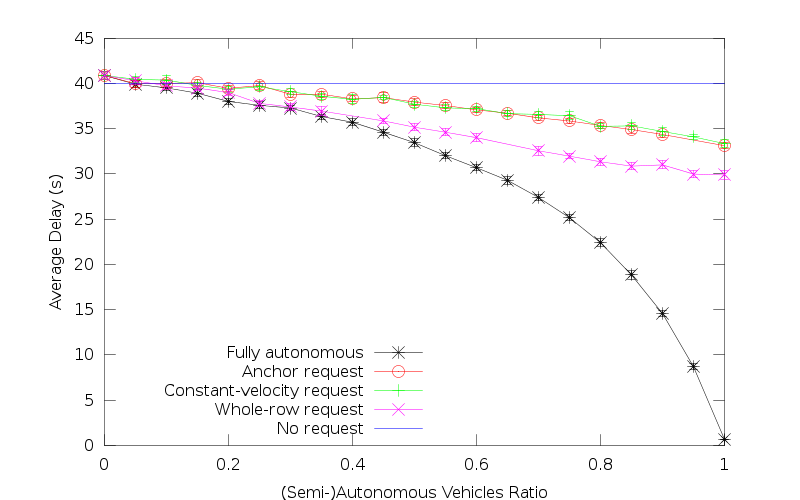
\includegraphics[width=0.8\columnwidth]{figures/figure_2.png}
% \caption{(Semi-)Autonomous vehicles vs. Human-Driven vehicles, traffic
% level = 360 vehicles/lane/hour.}
% \label{fig:two360}

% Figure~\ref{fig:figure1} shows that as the number of autonomous
% vehicles increases, the average delay decreases. In particular, when
% most vehicles are autonomous, the average delay is close to zero.  In
% the second experiment, we created a traffic consisting of
% human-controlled vehicles and two kinds of semi-autonomous vehicles
% but no autonomous vehicles.  We measured the average delay of all
% vehicles when we gradually increased the percentage of semi-autonomous
% vehicles.  Then we compared SemiAIM with optimized traffic signals.
% The results in Figure~\ref{fig:two360} shows that as the number of
% semi-autonomous vehicles increases, the average delay decreases under
% SemiAIM.  While the decrease is not as dramatic as the decrease when
% the percentage of autonomous vehicles is near 100\% in
% Figure~\ref{fig:figure1}, SemiAIM can reduce about 43\% of the average
% delay when most vehicles are semi-autonomous.



%%% Local Variables: 
%%% mode: latex
%%% TeX-master: "main"
%%% End:
